% @Author: AnthonyKenny98
% @Date:   2020-02-29 17:30:44
% @Last Modified by:   AnthonyKenny98
% @Last Modified time: 2020-04-03 14:28:30
\begin{figure}[H]
\begin{center}

    % Subfigure A
    \begin{subfigure}{\textwidth}
    \begin{center}
    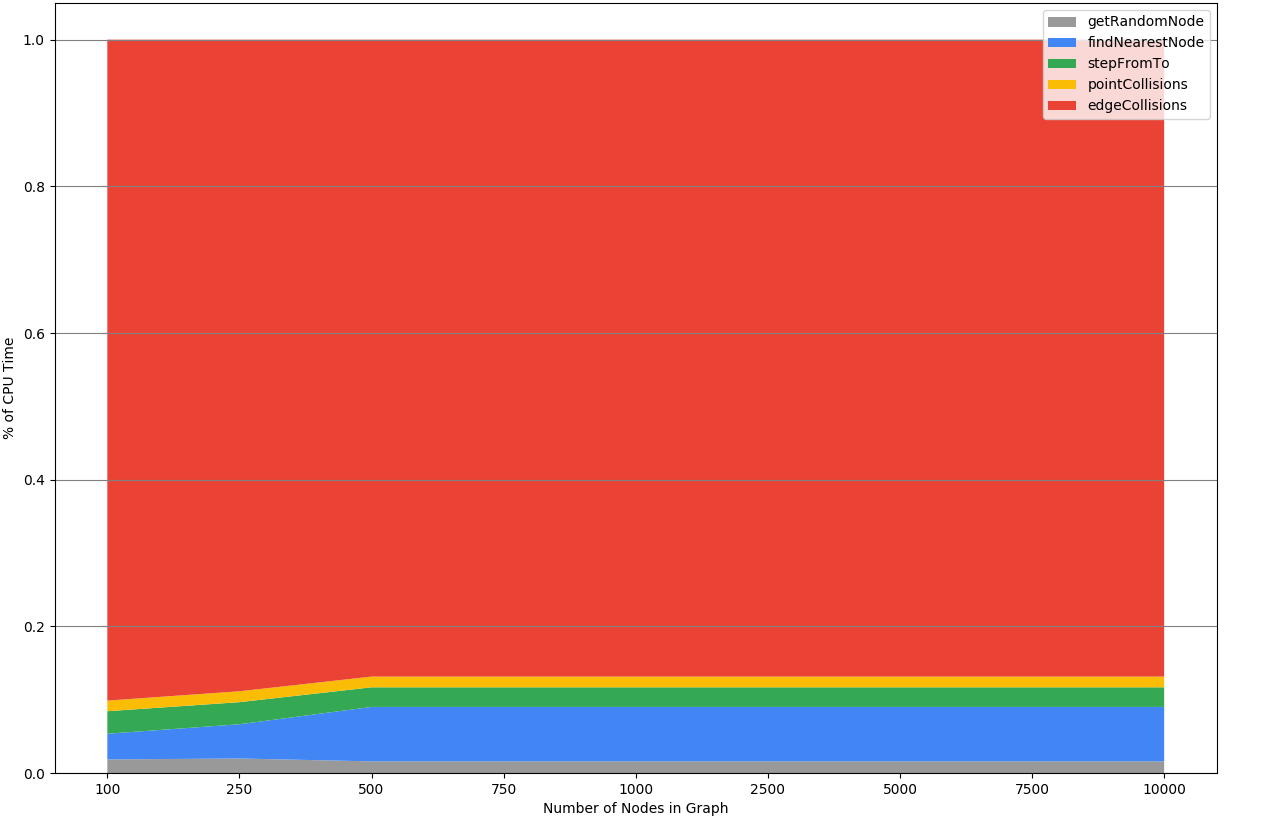
\includegraphics[width=\linewidth,height=0.3\paperheight]{chapters/chapter2/img/profiling/16x16x16/performance2.png}
    \caption{16x16x16 \gls{configuration} Space}
    \label{subfig:16x16x16rrt2}
    \end{center}
    \end{subfigure}
    % 
    % Subfigure B
    \begin{subfigure}{\textwidth}
    \begin{center}
    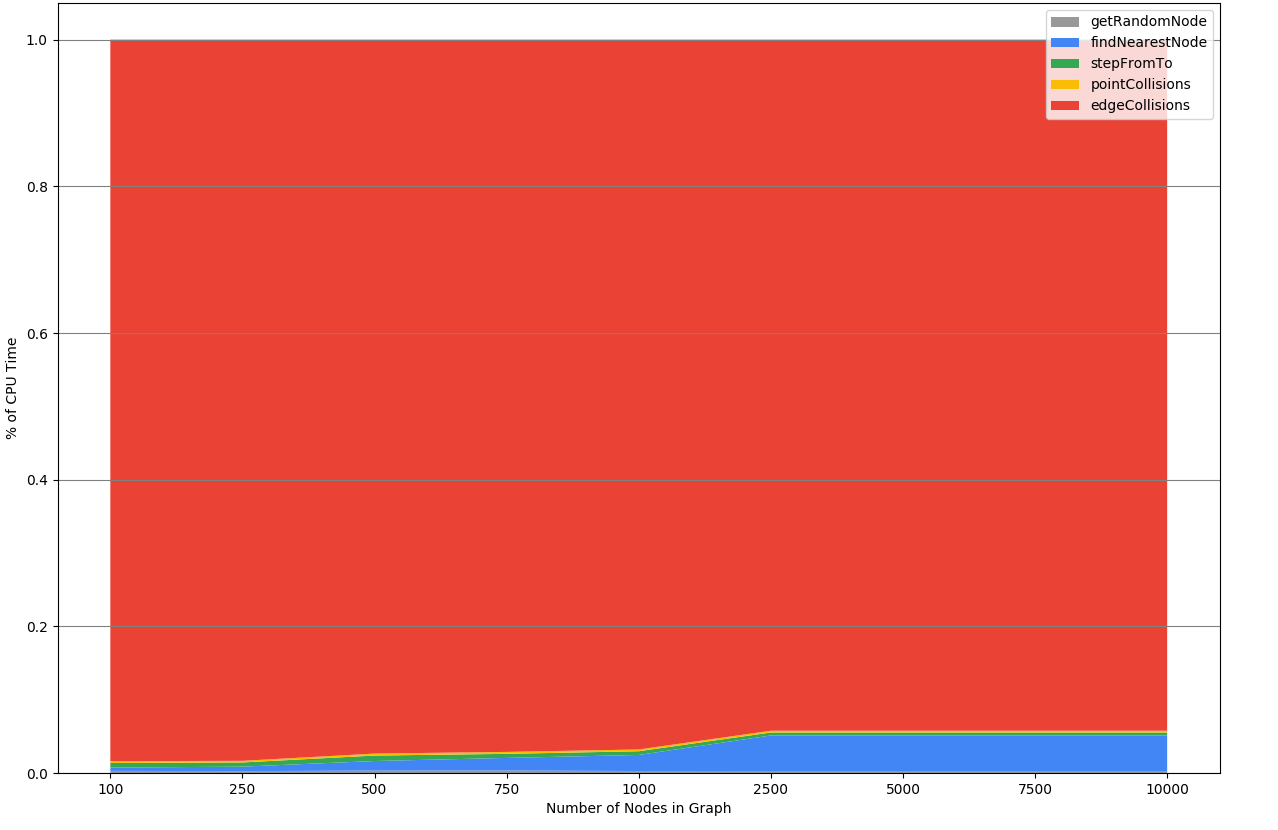
\includegraphics[width=\linewidth,height=0.3\paperheight]{chapters/chapter2/img/profiling/32x32x32/performance2.png}
    \caption{32x32x32 \gls{configuration} Space}
    \label{subfig:32x32x32rrt2}
    \end{center}
    \end{subfigure}
    % Caption and Label
    \caption{\gls{RRT} Functions Exectution Time, with Bucket Optimization}
    \label{fig:rrt_profiling2}
\end{center}
\end{figure}